\section{Periodic table}

\begin{figure}[H]
  \centering
  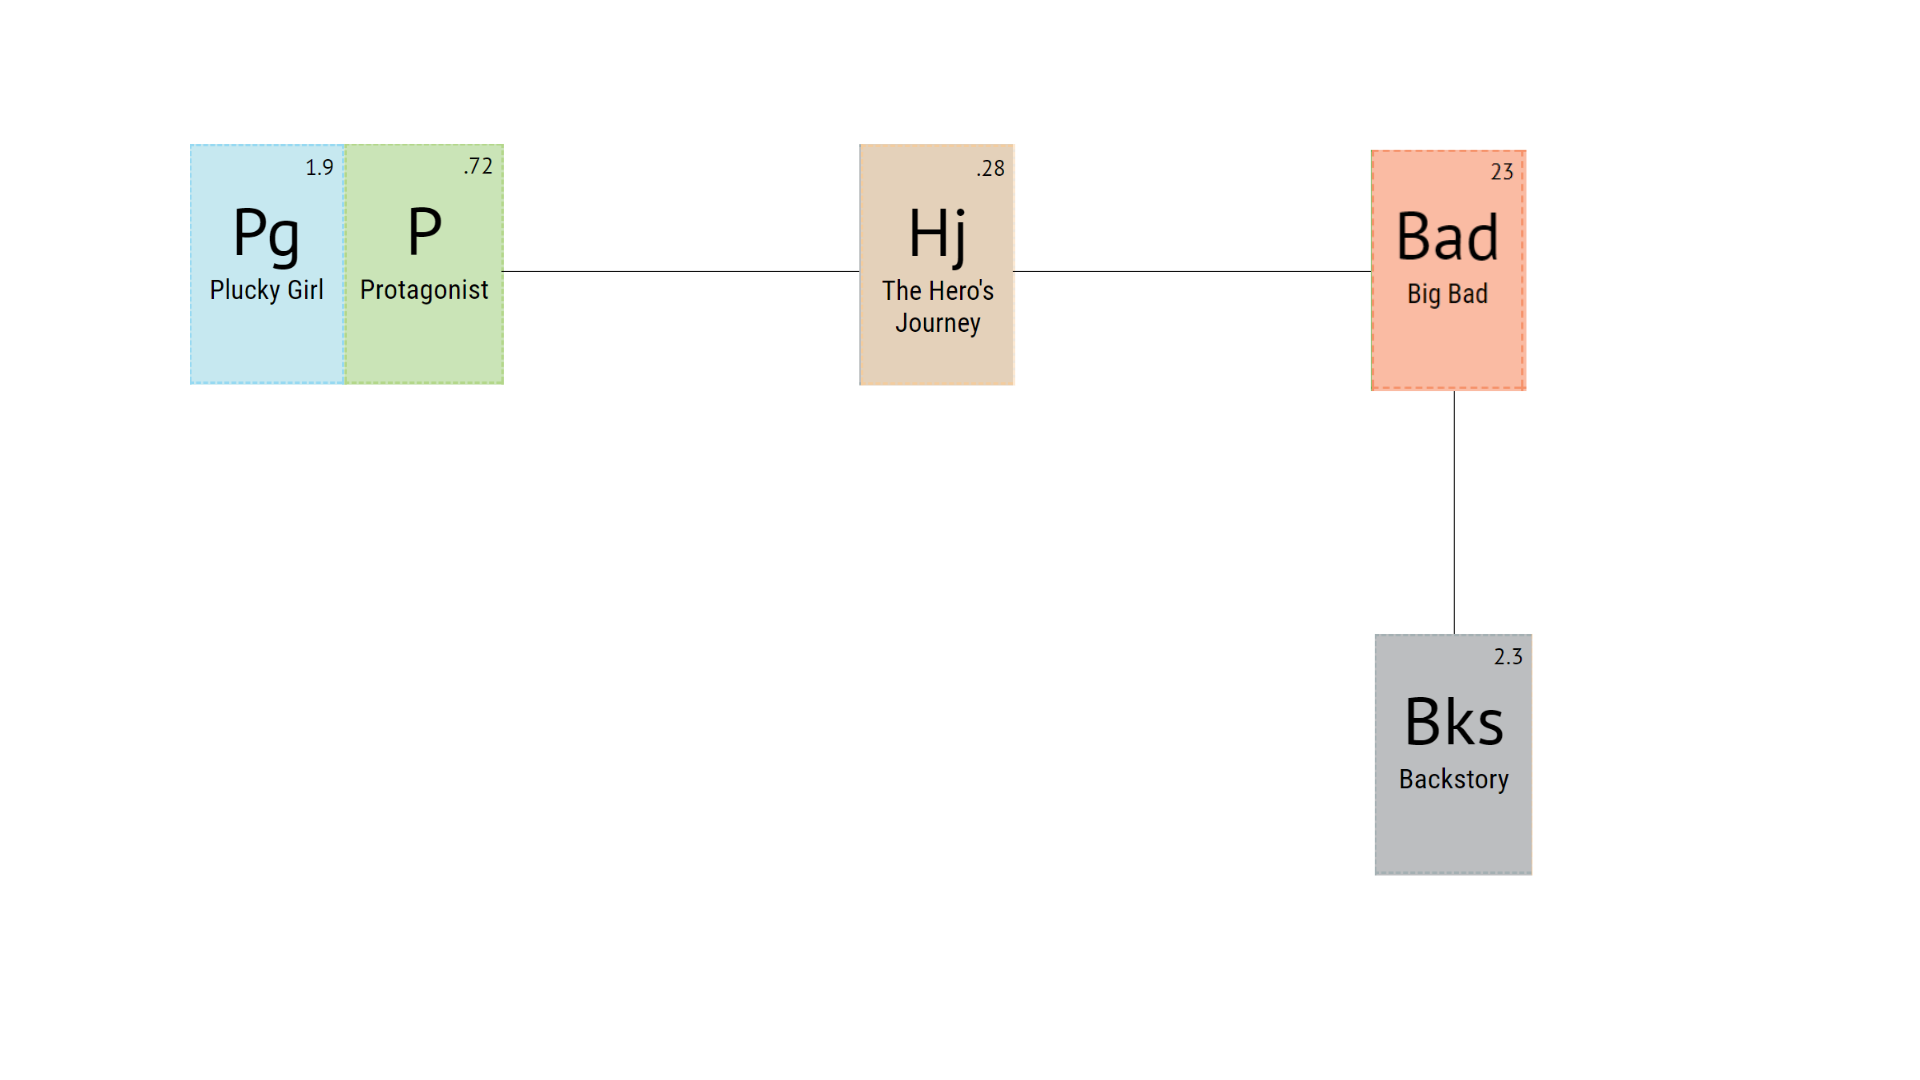
\includegraphics[width=\textwidth]{Images/Diagrams/periodicTable}
  \caption{Tropes form the periodic table of storytelling}
\end{figure}

\begin{itemize}
\item Pg-P: the protagonist is a brave and optimistic girl. In the course of the story, she will demonstrate her tenacity and her abilities in order to save her beloved.

\item Hj: the story is based on the Hero's Journey pattern described by Joseph Campbell. The journey of the protagonist come with a call to adventure (her beloved is missing) and will finish with a homecoming.

\item Bad: the main antagonist is the cause of all bad happenings in the story.

\item Bks: the background story explains the fundamental reason why the main antagonist has turned evil.
\end{itemize}
